\documentclass[preview, american]{standalone}

\usepackage[siunitx]{circuitikz}

\ctikzset{bipoles/capacitor/height/.initial=.4854}
\ctikzset{bipoles/capacitor/width/.initial=.1}

\begin{document}%
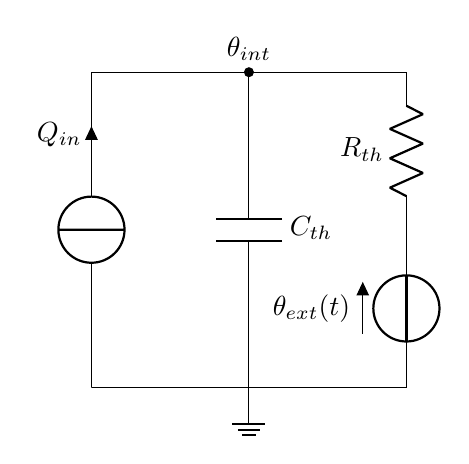
\begin{tikzpicture}
  \draw
  (0,0) to[current source=\(Q_{in}\)] (0,4)
        -- (2,4)
        to[C=\(C_{th}\)]  (2,0)
        -- (0,0)
        -- (4,0)
        to[voltage source=\(\theta_{ext}(t)\)] (4,2)
        to[R=\(R_{th}\)] (4,4)
        -- (2,4)
        
  (2,-0.05) node [ground] {} to (2,0)
  
  (2,4.3) node {$\theta_{int}$}
  
  (2,4) node [circ] {}
        ;
\end{tikzpicture}
\end{document}